\section{Introduction}
Experiment management in any domain is challenging.  There is a perpetual
feedback loop cycling through planning, execution, measurement, and analysis.
The lifetime of a particular experiment can be limited to a single cycle 
although many require myriad more cycles before definite results can be 
obtained.  Within each cycle, a large number of \Term{\subs} may be executed
in order to measure the effects of one or more independent variables.  

Experiment management in high performance computing (HPC) follows this general
pattern but also has three unique characteristics.  One, computational science
applications running on large supercomputers must deal with frequent platform
failures which can interrupt, perturb, or terminate running experiments.  Two,
these applications typically integrate in parallel using MPI as their
communication medium; each \sub\ within HPC is typically executed with an
\Term{mpirun} command.  Three, there is typically a scheduling system (\eg\
Condor, Moab, SGE, \etc) acting as a gate-keeper for the HPC resources.

In this paper, we introduce \namefull\ (\name), an experimental management
framework simplifying all four phases of experiment management.  \name\
simplifies experiment planning by allowing the user to describe their
experimental goals without having to fully construct the individual parameters
for each task.  To simplify execution, \name\ dispatches the \subs\ itself
thereby freeing the user from remembering the often arcane methods for
interacting with the various scheduling systems.  By providing
\Term{transducers}, \name\ automatically measures and records important
information about each \sub; these transducers can easily be extended to
collect additional measurements specific to each experiment.  Transducers are
implemented as wrappers that execute each \sub\ and can be extended to parse
the output of each \sub;  the term is borrowed from a similar concept in
Semantic File Systems~\cite{gifford-sfs}.  In both \name\ and Semantic File
Systems, transducers automatically generate semantically meaningful information
in \kv\ pairs which can then be easily searched.  Finally, experiment analysis
is simplified by providing \dbviz\, a general database visualization framework
that allows users to quickly and easily interact with their measured data.
\dbviz\ provides two important advanced features for improving data analysis:
\Term{outlier analysis} and \Term{hidden difference search}.  A typical
experiment workflow is shown in Figure~\ref{typical}; Figure~\ref{lem-plan}
shows the same workflow augmented with the various components of \name.

Although our experiment management framework has been designed for use at Los
Alamos National Lab (LANL) and therefore generally for an HPC environment, we
believe it can be easily modified to be suitable for experiment management in a
Grid environment as well.  Throughout this paper, we discuss how \name\ reduces
the complexity of managing experiments that may span multiple supercomputers
and the different scheduling systems on each.  In terms of experiment
management, supercomputers in HPC are very similar to clusters in the Grid.
Although the Grid introduces additional complexity due to multiple
administrative domains, we believe that \name\ can be useful in this
environment as well but this is not a focus of this paper.

\begin{figure*}[tb]
    \centering
    \subfloat[\label{typical}Typical Experiment Lifecycle]{
        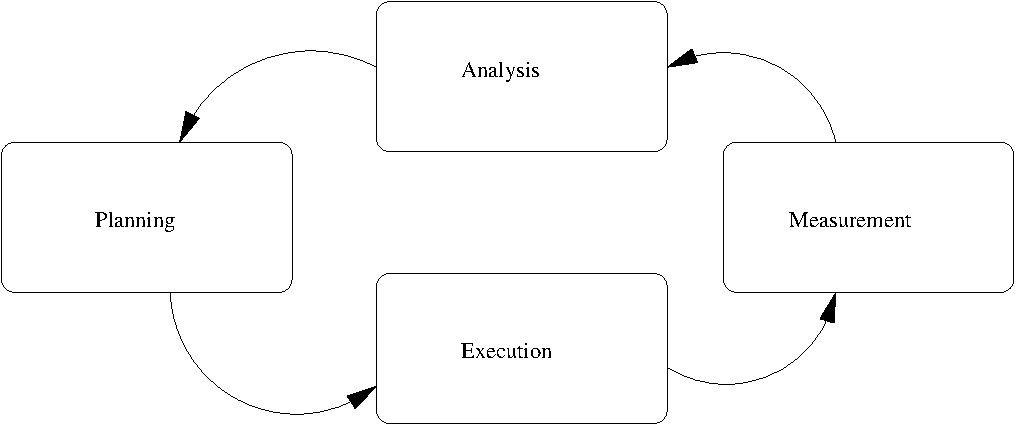
\includegraphics[width=0.4\textwidth]{figs/planning.pdf}
    }
    \hspace{0.5in}
    \subfloat[\label{lem-plan}\name\ Augmented Experiment Lifecycle]{
        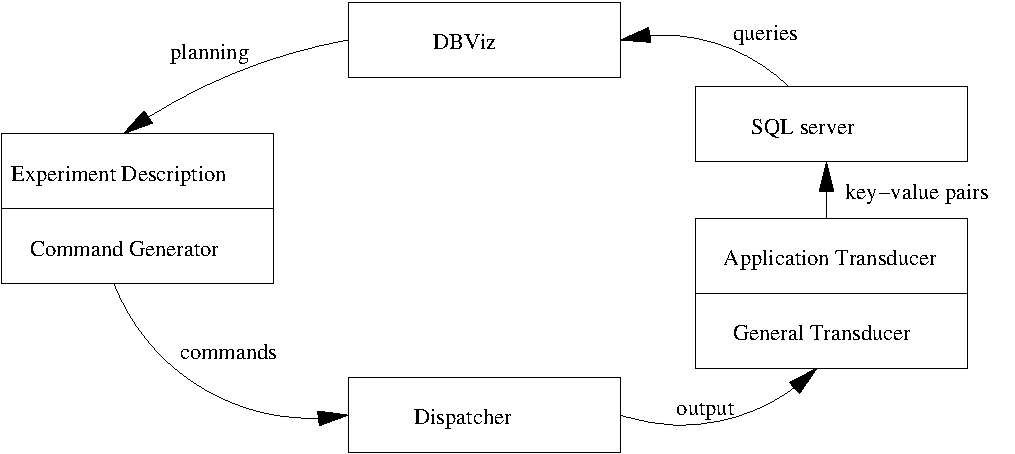
\includegraphics[width=0.4\textwidth]{figs/arch.pdf}
    }
    \mycaption{fig-plan}{Experiment Lifecycle.}{
The figure on the left depicts a typical experiment lifecycle progressing
through planning, execution, measurement, and analysis.  A user devises an
experiment to study the effect of some number of independent variables,
executes and measures each \sub, analyzes the results, and, depending on that
analysis, can then revise the experiment and repeat the cycle.  The figure on
the right shows the workflow within \name.  The user describes their parameter
space to the \cg\ and specifies a path to an optional application transducer to
capture application specific \kv\ pairs.  \name\ adds a path to a general
transducer to capture \kv\ pairs common to all experiments.  The generated
commands and their transducer(s) are then passed to the \dispatcher\ which
either submits the commands to a scheduling system or runs them synchronously
in the foreground.  As the commands run, \kv\ pairs are captured by the
transducer(s) and inserted into a SQL server from which they can then be
queried to visualize and analyze the results.  Depending on this analysis the
user can then modify their parameter space and repeat the cycle.
}
\end{figure*}


The remainder of the paper is organized as follows.  We describe our design in
Section~\ref{arch}.  In Section~\ref{eval}, we offer a demonstration of our
usage model.  We provide a comparison to related work in Section~\ref{related},
current status and future work in Section~\ref{future}, and a conclusion in
Section~\ref{conclude}.
